\documentclass[12pt,a4paper]{article}
\usepackage{amsmath}
\usepackage{textcomp}
\usepackage[a4paper,margin=0.8in]{geometry} 
\usepackage{natbib}
\usepackage{longtable}
\usepackage{graphicx}
\usepackage{appendix}

\bibliographystyle{agsm}

%opening
\title{An investigation into use of machine learning techniques as a tool in the study of the factors that affect life expectancy on a global scale}
\author{Adriaan Louw (53031377)}

\begin{document}

\maketitle

\newpage

\thispagestyle{plain}
\begin{center}
    \Large
    \textbf{Abstract}
\end{center}


The pursuit of increasing ones life expectancy is a very human endeavour. This study examines the tools used to study the conditions that affect life expectancy of countries. Investigating socio-economic indicators like income, educational attainment and per capita spending on healthcare. Understanding these relationships can lead a country to better a understand of which socio-economic areas to focus on, in order to increase their life expectancy. For this task this study advocates the use of certain machine learning algorithms that could be of greater use than the traditional regression techniques used in research.

\newpage

\tableofcontents

\listoffigures

%\listoftables

\newpage

\section{Introduction}

Human beings have always had a fascination with longevity. Myths like the fountain of youth or the Holy Grail are a testament to this fact. Today, longevity and causes of mortality are studies by professionals like Demographers and Actuaries. Trying to determine why some people or group live long lives.    

This study investigates the use of Machine Learning techniques in studying determinants of life expectancy for countries. Indicators that have shown to have some form of correlation with life expectancy will be selected. Their relationship with life expectancy will be investigated using various techniques from Machine Learning and contrasted to various forms of regression whose use is ubiquitous in the literature. This analysis will seek out to prove the appropriateness of using these machine learning algorithms for use in research to find the exact correlation between these indicators and life expectancy. It is the hypothesis of this study that machine learning techniques like k-Nearest Neighbour and Support Vector Machines will model the indicator/life expectancy relationship better than regression techniques can. Also that these techniques can create more accurate models. In the hope that the causes of long life expectancies in certain countries can be better understood \citep{Chen2017}. This study does not aim to prove causation between the indicators chosen and life expectancy, but rather the usefullness of machine learning algorithms as  tools. 

Statistical regression techniques are predominantly used algorithm for data analysis. Linear regression (Section \ref{regression}) forinstance assumes a linear relationships between the independant variables and the dependant variable. Which might not be the case. This we will discuss in Literature Review (Section \ref{lit}).

\section{Literature Review} \label{lit}

Life expectancy and mortality are 2 related terms. Mortality is generally expressed as a mortality rate. It describes the rate at which people die under certain circumstances. Life expectancy (Section \ref{LEXP}) is the amount of years an individual or group of people are expected to live. If the amount of people who are dying increases, the mortality rate increases and the life expectancy for people in that group decreases and visa versa.

\subsection{What do we mean by life expectancy?} \label{LEXP}

A life table is a table given for a specific year that contains the probability that a person of a certain age will die in that specific year. Acuataries and Demographers use life tables in the insurance industry and the study of demographics respectively. Life expectancy is one element of a life table. Both countries and the United Nations create life tables for use in policy creation.

There are 2 types of life tables, namely period and cohort life tables. A cohort is a group of people who were born in the same year. A cohort life table will follow a cohort over its lifetime until every member of the cohort has died. A cohort life table requires the mortality information of the cohort over many years. This information is often unavailable. While for a period life table, a hypothetical cohort is created and subjected to current mortality rates. This gives the user of the period timetable a window to see mortality rates at that point in time. This makes period life tables the most common type \citep{Arias2017}. 

A life expectancy figure from a period life table is called a period life expectancy.

\subsection{Multi indicator studies}

In this section, studies that used various indicators will be discussed.

\cite{Kabir2008} investigated how well the life expectancy of 93 developing countries were predicted by indicators like income,education and fertility (among others). It classied a countries life expectancy into 3 categories. Then used a probit model where the input variables have a linear relationship. Multiple Ordinary Least Squares Regression was then applied to study inicators' influences.

The study \cite{Hu2015}, also used a linear regression model of GDP per capita, Gini indeces, ect with respect to life expectancy. The intention of the study was to link income inequality to mortality rates and life expectancy.

While \cite{Shaw2005} investigated factors like smoking, pharmasutical spending, amount of butter consumed and amount of fruit and vegetables consumed. Then putting them in a linear model and applying regression.   

In an examination of 108 countries, \cite{Hassan2016} investigated indicators like education, GDP and health spending as it relates to life expectancy. They used Grossmans model \citep{Grossman2000}  
to model their data and Vector Error Correction Model to anlyse the data.

By using the componets of the Human Development index and Pearsons r with multivariate regression, \cite{Bulled2010} investigated the link between life expectancy, education and reproduction.

This study aims to add machiine learning algorithms as a tool to life expectancy studies, like these, that look at multiple factors that affect life expectancy.





%\subsection{Multi variate studies}

\subsection{Determinants of life expectancy}

This section summarises the relationship some indicators have with life expectancy.

\subsubsection{Income} \label{income}

The relationship between life expectancy and income has been given a lot of attention in academic circles \citep{Preston1975, Hu2015, Chetty2016, Oeppen2019}. 

\cite{Preston1975} was the first to show the correlation between life expectancy and per capita income. His original curve can be seen in Figure \ref{Preston}. As we can see from Figure \ref{Preston}, for low income countries, life expectancy increases rapidly with per capita income. Whereas in high income countries a small increase in per capita income does not have a large effect on life expectancy.

This relationship has also been shown in more recent studies \citep{Chetty2016,Oeppen2019}. Even though \cite{Shkol2019} found that in Russia, the Preston curve is not an accurate predictor of life expectancy, they found that the actual life expectancy should be ``substantially higher'' when comparing to the Preston curve predicted value. 

Studies in first world countries involving mortality rather that life expectancy have also found a relationship with income level \citep{Blakely2004,Kalwij2013,VonGaudecker2007}.

Just 16\% of the improvement in life expectancy between the 1930s and 1960s could be explained by rising income levels \cite{Preston1975}. Which seems to indicate that a countrie's life expectancy is dependant on more than income levels.  

\begin{figure}
\centering
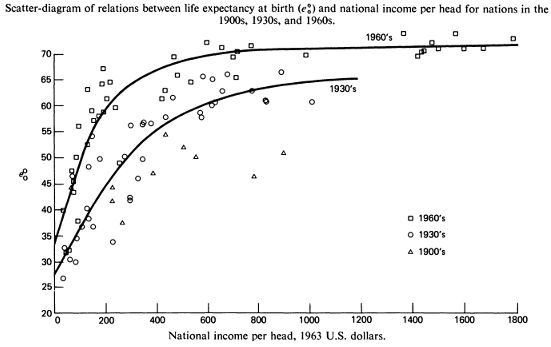
\includegraphics[ height=9cm, width=13cm]{The-original-Preston-Curve-1975.jpg}
\caption{The original Preston curve from \cite{Preston1975}}
\label{Preston}
\end{figure}

\subsubsection{Education attainment}

\cite{Kaplan2015} investigated the relationship between educational attainment and life expectancy in eight states in the United States. They found that even when controlling for variables like income, race, sex, and common medical issues like cardiovascular disease, the relationship between educational antainment and life expectance remains statistically significant.

\cite{Luy2019} studied 3 developed nations, namely the United States, Italy and Denmark. They have also found a strong correlation between education levels and longevity.

But what is the nature of this correlation? According to \cite{Deary2004}, Intelligence Quotient or IQ could explain the association. While \cite{Hayward2015} does not believe in a ``causal relationship'', but rather that it depends on factors like ``time, place, and the social environment''.

In an attempt to find a causal relationship between education and life expectancy, \cite{VanKippersluis2009} investigated the result of the Netherlands increasing the mandatory number of years a child had to attend school for to 7 years. It was 6 years previously. \cite{VanKippersluis2009} found a decrease in mortality of 3\% for 81-year old males who had the additional year of schooling. 

This relationship appears strongest in more developed countries where the life expectancy is already above 60 years \citep{Bulled2010}. In these countries, any educational investment leads to greater compensation for the learner than they would get in a less developed country \cite{Bulled2010,Handwerker1986}. In addition, \cite{Kabir2008} also studied this relationship, among others, with regards to developing countries and did not find a correlation. 

The literature appears not to be in agreement.

The question remains, which educational indicators should be used when investigating the relationship between education and life expectancy?

Various educational indicators have been used in the literature for comparing to life expectancy. One approach is to use the International Classification of Education (ISCED) system \citep{UNESCO2012}. The ISCED 2011 standard consists of 9 levels ranging from ISCED level 0 (Early childhood education) to ISCED level 8 (Doctoral or equivalent level).

\cite{Luy2019} used the United Nations ISCED-97 (consisting of 7 levels) scale to break education attainment down into 3 levels namely Low (None to Lower Secondary), Medium (Upper secondary) and High (Tertiary education). In \cite{VanKippersluis2009} the Dutch SOI system (Standaard Onderwijs Indeling). Which, according to \cite{VanKippersluis2009}, is similar to the ISCED system. While in \cite{Deboosere2009}, educational attainment was broken into 5 levels, also ranging from no education to Tertiarty education. 

\cite{Kaplan2015} broke educational attainment into 4 levels ranging from less than high school to college graduate.

In the study \cite{Bulled2010}, the relationship between educational investments and fertility against life expectancy, over 193 countries, was investigated. They used adult literacy and the enrolment ratios for primary,secondary and tertiary schooling.


%For more see \cite{Montez2015} Much information!!!!
%\cite{VanBaal2016a}

\subsubsection{Spending on health}

Healthcare spending and life expectancy in the Unites States, between 1960 and 2000, was compared in  \cite{Cutler2006}. They found that increased spending on health per capita, controlling for inflation, is positively correlated to US life expectancy for the time period in question. 

Most Eastern European countries, who have joined the European Union, have seen an increase in healthcare spending. This has generally been accompanied by an improvement in life expectancy \citep{Jakovljevic2016}. This has to be seen in the context of the so called ``Russian Mortality Crisis'' where former Soviet Union countries faced a sudden drop in life expectancy after the fall of the Berlin wall \citep{Brainerd2005}. \cite{Jakovljevic2016} found that the best metric to use when comparing health spending of countries, is to use their total per capita health spending (in US dollars).

The same relationship was found in Canada. When spending on healthcare is decreased, life expectancy follows \citep{cre}.

It is well known that life expectancy in Sub-Saharan Africa is low. Here spending on health care can also be correlated to increases in life expectancy. Even though poor governance can undo some of the effects of increased spending \citep{Makuta2015}.

A country's per capita healthcare is not necessarily in proportion to its per capita income. In 2005, the United States spent 50\% more on healthcare per capita than its income per capita would suggest \citep{Anderson2008}.






%Husain, AR (2002), �Life Expectancy in Developing Countries: A Cross-Section Analysis�, The Bangladesh Development Studies, 28(1&2)








%\cite{Shaw2005} showed that pharmaceutical expenditures shows a positive correlation with life expectancy in OECD countries.

%medical spending \cite{Cutler2006}

%?Grossman?
%2017 determinants of health: an economic perspective  ????
%1972 The Demand for Health: A Theoretical and Empirical Investigation,

%\cite{Grossman2000}

\subsubsection{Unemployment}

According to \cite{Bonamore2015}, the literature has 2 main views on the relationship between unemployment and life expectancy. The first view states that during an economic downturn, people suffer from more stress and depression. This leads to more unhealthy lifestyle choices like smoking and alcohol. Which in turn lowers life expectancy. \cite{Bonamore2015} cites the works of \cite{Lundin2014,Montgomery2013,GARCY20121911,BROWNING2012599,valos2012,backhans2011unemployment,DEB2011317} and \cite{Strully2009}, who take this view. The second view focusses on times when there is economic growth, i.e. less unemployment. This period of economic growth also can lead to stress eg. burning out and having less time for activities that benefit ones health. Like going to the gym. This view is held by \cite{TapiaGranados2011,RUHM2005341,TapiaGranados2005,NEUMAYER20041037} and \cite{Ruhm2000}. Then there are also studies express the view that no connection can be established \citep{Bonamore2015}. The view of  \cite{Bonamore2015} is that this relationship is non-linear.


%unemployment \cite{Bonamore2015} \cite{Roelfs2011} \cite{Roelfs2015} 

\section{Methodology/Procedure}


This study will attempt to create a model that can predict life expectancy for a country based on various socio-economic conditions in the country over a 30-year period. Then evaluate how well various machine learning techniques model these relationships. Unlike \cite{Shaw2005}, this study will not take into account the age distribution of each country.

The philosophical standpoint of this study is Positivism. By using the scientific method, this study will comprise of an experiment to inductively determine whether machine learning techniques can provide more accurate life expectancy models than those created using regression. This cross-sectional study will use life expectancy indicators shown, from the literature, to have some correlation to life expectancy.

Firsly appropriate data sets will be chosen. Taking into account that some indicators might have sparse information. This will impact the size of the dataset. Looking at available indicators like \cite{adultLiteracy}, we can see there are approximately 200 countries. If all the indicators have data for each year in the study there will be around 6000 data points. Looking at indicators like \cite{adultLiteracy} and \cite{pphealthspending}, it is clear that the data is quite sparse, especially for developing countries. The intention is to have the study encompass developed and developing countries, but this will depend on data availability.

Once the dataset is finalised, the algorithms and their permutations described in Section \ref{algo} will be applied. Three models will be created for each algorithm and permutation thereof. The first model will be using all the data. The second will only use data from developed countries and the third will only use data from developing countries, data permitting. Cross-validation will be applied to the created models as described in Section \ref{cross}.

The results from the regression analyses will then be compared to the results form the machine learning algorithms and that from the literature review above. 

\subsection{Choice of dataset}

\subsubsection{Life Expectancy}
For life expectancy data, this study will use the indicator ``Life expectancy at birth, total(years) \{SP.DYN.LE00.IN\}'' from the World Bank's Development Indicators Database \citep{WDI}. This is a weighted average combining both male and female life expectancy and is calculated in a period life table (see Section \ref{LEXP}). Only the data that is available for the last 30 years (1981-2010) will be used. This is in keeping with other studies where the amount of years that their studies look back on is limited to relatively recently \citep{Luy2019, Hu2015,Tarkiainen2012,Kabir2008, Shaw2005}. 

\subsubsection{Income}

This study will use GDP per capita as was used in \cite{Oeppen2019,Shkol2019,Mackenbach2013} and \cite{DeVogli2005}. The source will be GDP per capita, PPP (constant 2011 international \$)\{NY.GDP.PCAP.PP.KD\} from the World Bank \citep{WorldBank_gdp}.

\subsubsection{Educational Attainment} \label{edudata}

This study will use the same indicators and was used in \cite{Bulled2010}. For an adult literacy indicator, SE.ADT.LITR.ZS will be used from the world bank website \citep{adultLiteracy}. This indicator describes the percentage of adults, from the age of 15, who can read and write to a certain level of proficiency. Determining the literacy level of a country is a difficult endeavour. The definition of literacy might be exactly the same between countries, because this indicator uses a lot of data that each country determines on its own. This also might include some measure of competancy with numbers.

The indicator SE.PRM.ENRR will serve as the enrollment ratio for primary education \citep{worldbankenrollmentprimary}. As the name suggests, it is the pecentage of students in primary school. It is calculated as the fraction of students in primary school over the amount of students that should be in prmary school basaed on population figures. This can lead to a value greater than 100\%. This is due to older students or adults that should have completed primary school that are now undergoing primary school education. This can be a sign of a poorly performing school system. This indicator also does not take issues like truancy into account. 

For secondary school enrolment, SE.SEC.ENRR  \citep{worldbankenrollmentsecondary} will be used. This   indicator can be higer than expected or above 100\% for the same reasons as the primary school enrollment indicator. 

SE.TER.ENRR \citep{worldbankenrollmenttertiary} will be used for tertiary enrollment. A high number here tends to indicate that it is a number from an developed country, because tertiary education is much more of a luxury in developing countries.

It is expected that the enrollment at tertiary and secondary will be highly correlated to industrialised countries and thus with life expectancy. The world bank credits \cite{UNESCOInstituteofStatistics2019} for all of theses educational indicator data.

\subsubsection{Per Capita spending on health}
To represent Per capita spending on health in this study's model, SH.XPD.CHEX.PP.CD \citep{pphealthspending} which describes Current health expenditure per capita, will be used.

\subsubsection{Unemployment}
Unemployment will be ignored for this study because sufficient data on unemployment per country is not available. This can be seen by looking at indictors like SL.UEM.TOTL.NE.ZS \citep{unemploymentdata} which describe percentage unemployment per country for both sexes.

\subsection{Choice of algorithms} \label{algo}

In this study Linear Regression will be used as a baseline for comparison on the dataset.

\subsubsection{Algorithms Chosen}
\paragraph{Linear Regression} \label{regression}
Linear Regression is a popular technique, used to find relationships in data. As the name suggests Linear Regression assumes a linear relationship between the input variables and the result \citep{Murphy}. This might not be the case for the target function. The target function could be any potential function. In the case of life expectancy modelling, we know that according to the Preston curve (Section \ref{income}), the relationship between income and life expectancy is not linear. Thus using Linear Regression should return a sub-optimal result unles the data is transformes using some non-linear function into a linear space. Linear regression was used in the following studies: \cite{Chetty2016,Jakovljevic2016,Hu2015,Mackenbach2013,Bulled2010}. 

\paragraph{k-Nearest Neighbour}

The k-Nearest Neighbour algorithm (kNN) is an instance based form of machine learning. It uses the classification of those datapoints closest to the data point to be classified to determine its classification. The kNN-algorithm allows for non-linear problem spaces to be classified, because it does not make an assumption on the nature of the problem space. It just sees a data point as a function of its closes neighbours. This is usefull for indicators like income that are highly non-linear as described in Section \ref{income}. Additionally, how the algorithm determined its output value is transparent and can be used to study how various components affect the end result. This is important , because if the algorithm was not transparent it can not be seen as a replacement for other algorithms that are transparent like regression alorithms. In this study, the standard kNN-algoritm will be altered to accomodate a real valued output and not just a class classification. This will be accomplished by taking the mean life expectancy for all the data points determined to be closest to the target point. Care will have to be taken to reduce the number of features of the data, because this algorithm is sensitive to the so-called ``curse of dimentionality'' \citep{Mitchell}. As discussed in Section \ref{edudata}, educational attainment will comprise of many indicators. This could lead to educational attainment being weighted more than other indicators. Thus each educational indicator will be given a fractional weight. If there are 4 educational attainment then each indicator will have a 4th of the weight of other indicators. 

The value of $k$ will have to be found experimentally and will be affected by the density of the data points. One potential issue could be if the data tends to cluster around certain points. This could happen if developing countries clster together and developed countries cluster together. That could make developing countries, that are on the higher end of the development scale, more difficult to classify, since not a lot of data points will be very close to them. 

\paragraph{Support Vector Machines}

The classic Support Vector Machine (SVM) is used in classification tasks. It involves determining the decision surface with regards to the data points closest to the surface. This study will use a modified SVM algorithm that makes it useful for regression tasks. This is called Support Vector Regression (SVR). The SVR algorithm is described in \cite{smola2004}. The final model can be described as:

\begin{equation}
 f(x) = \sum_{i=1}^l (\alpha_i-\alpha_i^*)k(x_i,x)+b
\end{equation}

where $\alpha_i$ and $\alpha_i^*$ are Lagrange multipliers, $b$ is the bias and the term $k(x_i,x)$ is the kernel function. The kernel is a function to determine the similarity between 2 input vectors. Kernel functions are used to map a non-linear problem space into a smaller subspace where the features are linearly seperable. A kernel has to map from the dimension of the problem space down to 1 dimension. Instead if computing the dot product of 2 datapoints, we can replace it with a kernel that requires less computation. Various kernels will be investigated, including the Radial-basis function

\begin{equation}
 k(x_i,x) = exp(-\frac{\mid\mid x-x_i \mid\mid^2}{2\sigma^2})
\end{equation}

and the polynomial kernel

\begin{equation}
 k(x_i,x) = (x_i.x +1)^p
\end{equation}

Unfortunately, SVR models are difficult to analyse. Making it hard to determine how the input features of the model affect the output. In order for SVR to be seen as a viable alternative to multivariate regression, an appropriate technique has to be found that can assist in this dilemma. For purpose, this study will use the techniques described in \cite{USTUN2007299} to understand which input feature the SVR model deems most important for the modelling of our life expectancy problem space.

In the algorithm described in \cite{USTUN2007299}, a kernel matrix or Gram matrix has to be computed. This matrix $K$ will be of size $N X N$ and contains in each cell the kernel function corresponding to the input vectors of the same index such that

\begin{equation}
 K_{ij} = k(x_i,x_j)
\end{equation}

The vector of input data(I) is of size $M X N$ where $M$ is the number of input features and $N$ is the size of the dataset. The Correlation matrics(R) is calculated by correlating each row of I with each column in K. This gives a resultant vector R of size $N X M$. Now we have a measure of the impotance of each input to the kernel matrix. This resultant matrix is then converted to an image so that the relationships can be seen visually.

\paragraph{Clustering}

Clustering techniques are a form of unsupervised learning where the algorithm tries to group the data in a number of groups. In essence, classifying the data into categories. This cannot be easily compared to regression techniques. This study will rather follow the approach of Clustered linear regression(CLR) \citep{Ari2002}. In CLR, clustering techniques are used to break the dataset into clusters. Then apply linear regression to the datapoints in each cluster. In this way one linear regression model does not have to account for all data the data in the data set. Each regression model can be tailored to data similar to it, thereby increasing the chance of getting a good linear fit on the data. This technique also allows the researcher to gain information about the dataset. If the data is very clustered, it could mean that the promlem space in not very linear and that data tends to ``jump'' between clusters. Comparisons will be made to how the number of clusters affect the results from the regression analyses.

Various clustering algorithms exist. They can be classified into 2 broad groups. The first group is flat clustering. In this group, the algorithms break the data into various groups that have no hierarchy. In other words, there are no group of groups. The second type in hierarchical clustering \citep{Murphy}. 

Agglomerative clustering and divisive clustering are the 2 types of hierarchical clustering. Agglomerative clustering starts of withm each data point being a cluster and then combining clusters until some condition is reached. Divisive clustering adds all the datapoints to one cluster and then breaks them into smaller sub-clusters until some condition is met \citep{Murphy}.

The k-means algorithm will be used for clustering. It is flat clusterig algorithm. A number $k$ will be selected, and that will be the number of clusters the algorithm will attempt to find. Each cluster is assigned a centroid that devines the middle of the cluster. The number k will have to be found experimentally, but it should correspond to broad catagories these countries can be placed in with regards to life expectancy. Forinstance, we could assume that these countries can only be grouped whether they are developing or developed countries. Then k would be 2. Another possibility is to group the countries according to their geographical location. That assumes countries that are close geographicaly also have similar life expectancies. Then k can be 6. one for each continent, excluding antarctica. Further subdevisions are possible \citep{Murphy}.

Each cluster has an initial start point, i.e. the initial position of its centroid. The centroid will be randomly placed in the hypothesis space. Each data point is the assigned to the nearest centroid, determined by Euclidean distance. The centroids position will then by updated to be the mean of all its newly assigned datapoints. The algorithms then repeatedly updated the position of each centroid based on the closest data points, until the centroid stop moving. It is worth noting that the algorithm might not coverge to the optimum solution. Therefor multiple runs of this algorithm will be necessary \citep{Murphy}.

\subsubsection{Ignored Algorithms}
\paragraph{Logistic regression}
This regression is appropriate when the dependant variable is discrete, e.g. a yes/no answer. It also assumes a linear relationship between inputs. In contrast to linear regression, this linear sum is passed through the sigmoid function \citep{Murphy}. All of this makes it inappropriate for non-linear target functions and this study.

\paragraph{Neural Networks}
Even though Neural networks are capable of representing non-linear hypothesis spaces \citep{Mitchell}, they are not appropriate for this study for a couple of reasons. Firstly, the datasets that are available are not large enough. Neural networks typically require thousands if not tens of thousands of data points. Secondly, the amount of processing power and processing time required, will not be available to this study. Thirdly, the results of neural networks are hard to interpret. How the Neural Network came to its conclusion is not clear to the researcher. Which makes it unsuitable as a tool to study the relationship between life expectancy and its various indicators.

\paragraph{Decision Trees}

Traceability and understandability are some of the hallmarks of Decision Trees. These algorithms are suited problem spaces where the target function and the input attributes are discrete values. It is possible to approximate continuous input attributes by making a branch in the tree when a value is smaller or greater than some value, or is between some value. For functions where input attributes span over large ranges, this leads to very large and sub-optimum trees \citep{Mitchell}. Many decision tree algorithms exist, like ID3 and C4.5. The problem of determining life expectancy from socio-economic indices has a continuous target function output and continuous input attributes. Therefor, Decision Trees will be excluded from this study.





\subsection{Cross-validation} \label{cross}

By using stratified \textit{k}-fold cross validation, this study will aim to reduce the impact of the relative small dataset that will be analysed. This form of cross validation will ensure that when the validation set is chosen, no important data points are ignored for training. The data will be broken down randomly into \textit{k} subsets of equal size. Each data subset will also contain equal amounts of data points with low and high life expectancies, so that no dataset is completely towards one end of the data range. One data subset is chosen to be the validation subset and the remaining $\textit{k} - 1$ subsets are combined into the training set. The model is then trained on the training dataset andt its performance is measured against the validation subset. This is done \textit{k} times in order for each subset to be the validation subset. For each of the training runs the mean of the error will be calculated \citep{Mitchell,Murphy}. The value of \textit{k} will be dependant on the final dataset. 

%\section{Analysis}


%\cite{Murphy} p23 how to compare techniques
%\section{Conclusion}

%\section{Recommendations}


%\appendix
%\appendixpage

%\addappheadtotoc
\addcontentsline{toc}{section}{References}
\bibliography{mybib}



\end{document}
